\chapter{Synthèse de commande}
\label{chap:commande}
\section{Commande du système d'ordre 2}
\subsection{Rédaction du cahier des charges et démarche de réponse}
Après l'étude que nous venons de réaliser sur notre système, nous allons ici exprimé les attentes que doit réaliser la commande que nous allons implémenter. Nous souhaitons avoir : \begin{itemize} 
\item Erreur de position nulle.
\item Pas d'oscillations
\item Temps de réponse inférieur à 1 seconde.
\end{itemize}
La commande de notre système doit permettre d'asservir le système en vitesse, par rapport à une consigne. Pour respecter, nous allons réaliser un placement de valeurs propres par retour d'état.



\subsection{Calcul du retour d'état}
\label{sub:Calcul du retour etat}
Pour garantir les performances dynamiques souhaitées, nous allons appliquer un placement de pôles par retour d'état. Ce réajustement des valeurs propres de la matrice dynamique du système nous permettra de répondre aux attentes du cahier de charges si le choix de celles-ci est correct. De même, nous devons choisir des valeurs propres qui ne sont pas être trop éloignées de celles du procédé, pour ne pas être trop exigeant avec la commande et le système. Nous avons avec ces spécifications choisi les valeur propres suivantes :
\begin{equation}
\label{equation:valeurPropres}
\lambda = \begin{pmatrix}
-4 &-5
\end{pmatrix}
\end{equation}
La commande par retour d'état est une technique d'asservissement qui permet de modifier le signal d'entrée du système en fonction de la sortie mesuré et une référence. Cette nouvelle loi de commande s'écrit : 
\begin{equation}
u(t) = Ny_{ref}-Ky(t)
\end{equation} avec $N$ un gain de pré-compensation, $y_{ref}$ la vitesse de référence, $y(t)$ la sortie mesuré du système et $K$ le gain de retour. Si l'on applique cette loi à notre système en espace d'état, on obtient : 
\begin{align*}
\left\lbrace
\begin{aligned}
&\dot{X}(t) = (A-BK)X(t) + BNy_{ref}\\
&Y = CX(t)
\end{aligned}
\right.
\end{align*}
Ainsi la nouvelle dynamique du système est donnée par la matrice $A' = (A-BK)$ et doit admettre les valeurs propres que nous désirons appliquer à notre système. $A$ et $B$ étant des paramètres du système, nous allons utiliser le gain $K$ pour répondre à ce problème. Avec la fonction $place$ de MATLAB, nous sommes capable de concevoir ce vecteur $K$. 

\subsection{Observateur ordre plein sur modèle d'ordre 2}
Pour pouvoir réaliser notre commande par retour d'état, nous devons tous d'abord reconstruire l'ensemble des états du système dont nous n'avons pas accès. Dans notre cas, nous disposons d'une mesure de la vitesse $\Omega$ avec la tension de sortie $V_s$ mais aucune information sur la position $\Theta$, l'implémentation d'un observateur est donc nécessaire pour au minimum reconstruire cet état.\\
Nous préférons reconstruire $\Omega$ et $\theta$ à partir de $V_s$ et de l'entrée du modèle d'ordre 2 pour simplifier les calculs nécessaire à sa construction. Il est représenté par :
\begin{align*}
\left\lbrace
\begin{aligned}
&\dot z (t) = Fz(t) + Gy(t) + Hu(t)\\
&\hat x = Mz(t) + Ny(t)\\
&\epsilon = x-\hat{x}
\end{aligned}
\right.
\end{align*} où $x$ représente l'état du système, $\hat{x}$ l'état du système reconstruit et $\epsilon$ l'erreur d'estimation à un temps $t$. Nous souhaitons contrôler la dynamique de ce paramètres pour pouvoir estimer correctement notre système. Pour cela, nous nous interressons à : \begin{align*}
&\dot{\epsilon} = \dot{x} - \dot{\hat{x}}\\
&\Leftrightarrow \dot{\epsilon} = Ax +Bu - F\hat{x} - Gy - Hu 
\text{   en considérant }M=1 \text{ et } N = 0\\
& \Leftrightarrow \dot{\epsilon} = Ax - F\hat{x} - GCx + u(B-H)\\
& \dot{\epsilon} = (A-GC-F)x + F\epsilon + u(B-H)
\end{align*} 
Il vient alors $F = A-GC$ et $B=H$ pour obtenir $\dot{\epsilon} = F\epsilon$. Ainsi l'erreur d'estimation est autonome et ne dépend pas des entrées et sorties du système, et il vient $\epsilon(t) = e^{Ft}\epsilon(0)$. Les valeurs propres de $F$ vont ainsi déterminer la dynamique de l'erreur d'estimation, nous choisissons de les faire dépendre des valeurs propres désirées dans la partie \ref{sub:Calcul du retour etat} en les multipliant par 3, pour une convergence encore plus rapide. 

\subsection{Construction de l'asservissement}
Maintenant que l'observateur et le gain du retour d'état sont construits, nous allons les assembler ensemble pour commander notre système. Pour ce modèle du système bouclé, nous prenons comme vecteur d'état $X=\begin{pmatrix}
X&\epsilon
\end{pmatrix}^T$ et nous obtenons par construction :
\begin{align*}
\label{eqn:systemeEE2_bf}
\left\lbrace
\begin{aligned}
& \dot{X} = \begin{pmatrix}
(A-BK) & -BK\\
0& F
\end{pmatrix}X+\begin{pmatrix}
B\\0
\end{pmatrix}y_{ref} \\
& y(t) = \begin{pmatrix}
C & 0
\end{pmatrix}X
\end{aligned}
\right.
\end{align*} 
Cependant, nous souhaitons asservir le système avec la vitesse $\omega$, et la description de ce système bouclé va asservir le système en position à cause du changement de dynamiques de la position $\theta$. Pour prévenir à cette mauvaise commande, nous avons annulé le retour de la mesure de position dans le système bouclé. 

Le gain de pré-compensation $N$ peut maintenant être calculé à partir gain statique du transfert entre $Vg$ et $y_{ref}$ noté $G_{Vg/y_{ref}}$ : 
\begin{equation}
N = \frac{1}{G_{Vg/y_{ref}}}
\end{equation}
A partir de ce modèle, nous allons être capable d'éprouver la commande obtenu de manière théorique et avec une simulation SIMULINK.

\section{Validation de la commande}
\subsection{Validation théorique}
Pour commencer, nous allons identifier les valeurs propres de notre système \ref{eqn:systemeEE2_bf} afin de de connaitre les effets de l'observateur sur le retour d'état, même si a priori celui ci est autonome. Nous obtenons les $\lambda_i$ valeurs propres suivantes : $-5$, $-4$, $-15$ et $-12$. Nous remarquons que les $\lambda_i$ n'ont pas été modifiées : nous avons les valeurs propres désirées par la commande et nous avons celles désirées pour l'erreur d'estimation de l'observateur. 

\subsection{Simulation SIMULINK}
Pour compléter la validation de la commande, nous avons crée un prototype avec SIMULINK pour pouvoir simuler une réponse temporelle de la commande de notre système. La description du fichier se trouve en annexe \ref{Annex:SIMULINK_RE}. Nous observons sur les figures suivantes la réponse temporelle à une référence $y_{ref} = 1$ : 

\begin{center}
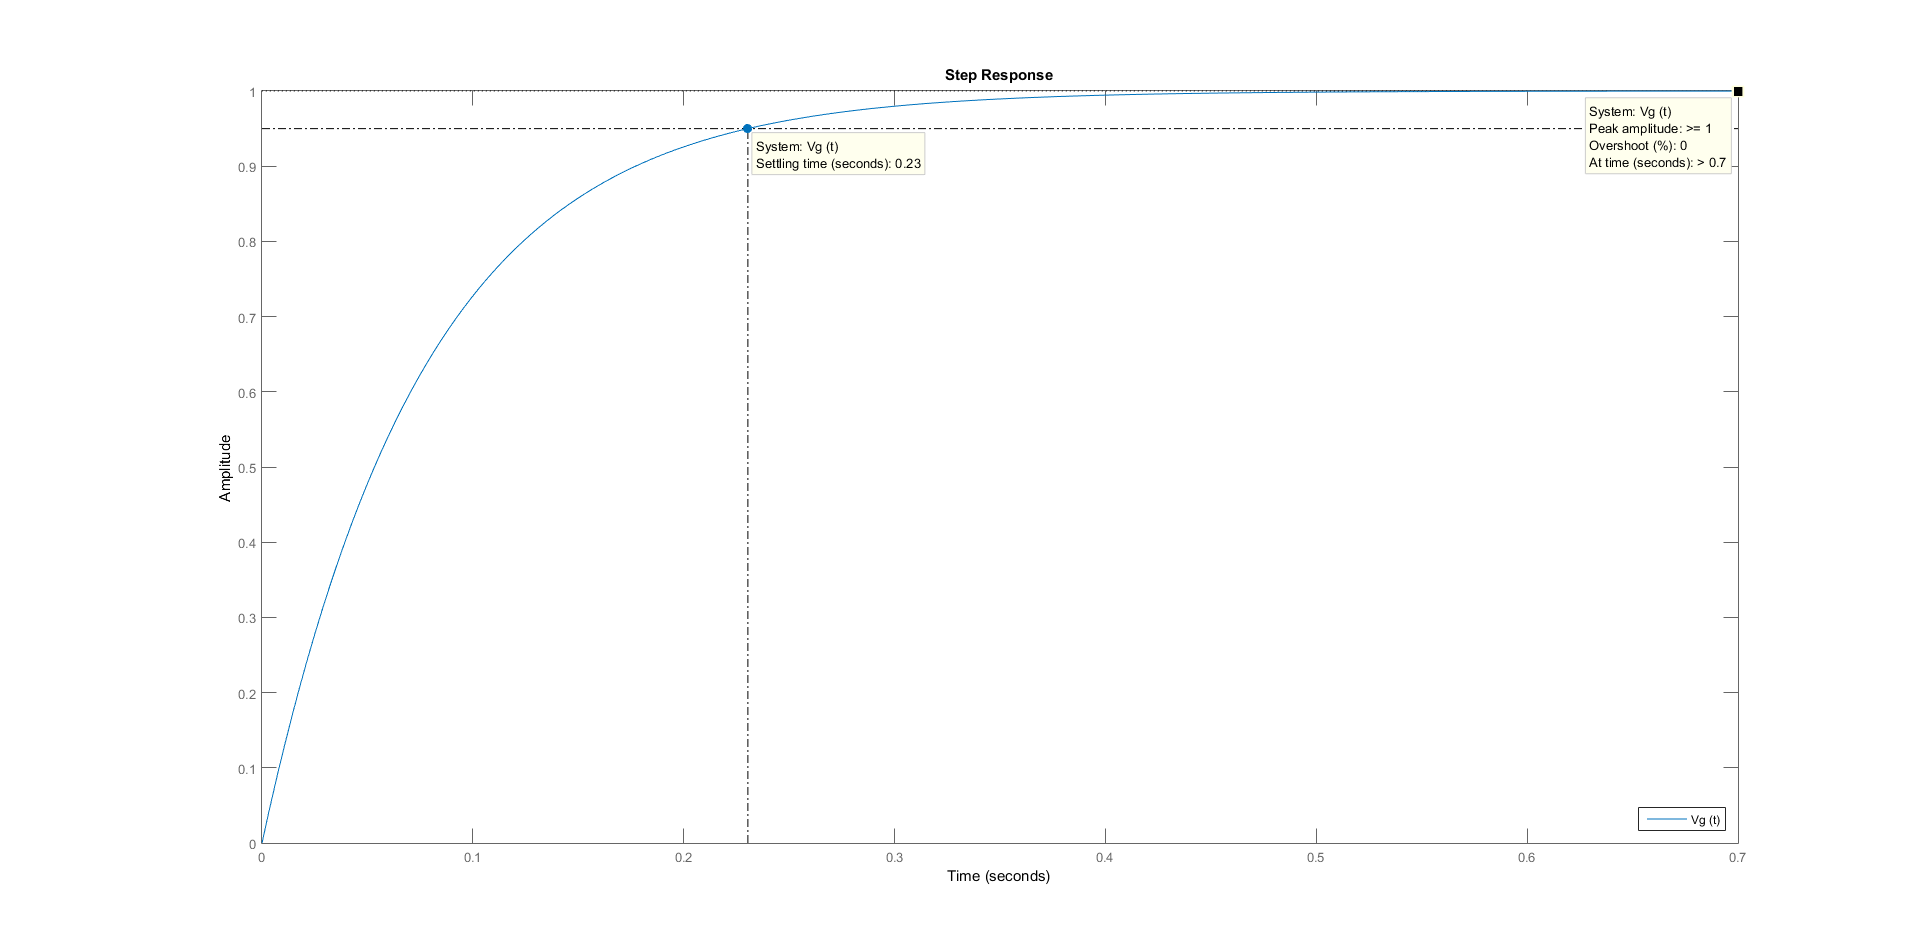
\includegraphics[width = \textwidth]{./III/figure/stepEE2bf.png}
\captionof{figure}{Réponse du système asservi}
\end{center}
La réponse du système $Vs$ simulé correspond aux changement de dynamique que nous avons espéré. De plus, après une observation de la commande $u(t)$ appliquée sur le système, nous voyons que la tension maximale envoyée est borné dans l'ordre de grandeur des valeurs admises par le système physique. 

\subsection{Analyse boucle fermé du modèle d'ordre 3}
Nous commande respecte le cahier des charges, nous validons ainsi la commande pour notre modèle d'ordre 2. Nous allons maintenant valider cette même commande sur des modèles supérieur et plus complexes pour compléter sa validation. En effet, notre modèle a été très simplifié pour permettre la création du commande facilement. Si nous arrivons a prouvé que cette commande marche sur des systèmes plus complexes, alors nous aurons prouvé que les dynamiques que nous avons simplifiés ne vont pas perturbé notre commande.

\section{Validation sur les modèles d'ordre supérieur}
Dans un premier temps, nous regarderons les effets de l'implantation de l'observateur d'ordre 2 sur les modèles d'ordre supérieur et plus précisément l'erreur d'estimation et le placement des valeurs propres, puis nous simulerons la commande obtenu pour observé les modifications des réponses.

Pour intégrer l'observateur dans un espace d'état d'ordre supérieur, nous avons du réorganiser les états du modèle, ici le modèle d'ordre 1, de façon à ce que les états reconstruits avec l'observateur soient en haut, $x_1$, et les non observable en bas $x_2$.

\noindent\textbullet\hspace{2mm} Etats observables : $\Omega_m$ et $ \Theta_m$.

\noindent\textbullet\hspace{2mm} Etat non observable : $i_1$

\noindent\textbullet\hspace{2mm} L'espace d'état est donc : 
\begin{equation}
\overline{X} = \begin{bmatrix}
\theta\\
\omega\\
i_1\\
\end{bmatrix} = \begin{pmatrix}
x_1\\x_2
\end{pmatrix}
\end{equation}
donc $x_1 = \begin{bmatrix}
\theta\\
\omega\\ \end{bmatrix}$ et $x_2 = i_1$. Pour passer de $X$ à $\overline{X}$, il faut utiliser une matrice de passage $P_X$ définit par :
 \begin{eqnarray}
 P_X &/&  \overline{X} =P_X \cdot X \\
 P_X &=&\begin{bmatrix}
 0 & 0 & 1 \\
 1 & 0 & 0 \\
 0 & 1 & 0 \\
\end{bmatrix}  \\
 \end{eqnarray}
Maintenant, nous devons calculer $\overline{A}$, $\overline{B}$, $\overline{C}$, $\overline{D}$ pour le nouvel espace d'état lié à $\overline{X}$.
\begin{equation}%
	\left\lbrace%
	\begin{matrix}
		\overline{A} &=& P^{-1} A P \\%
		\overline{B} &=& P^{-1} B \\%
		\overline{C} &=& C P%	
	\end{matrix}
\right.%
\end{equation}

Avec les résultats obtenus pendant les séances de TD et de cours, nous avons \begin{equation}
\dot{\epsilon} = F\epsilon - A_2x_2
\end{equation}
avec $A_2$ la partie qui lie les états $x_1$ et $x_2$ dans la nouvelle base. Cet élément modifie les résultats que nous avons obtenu pour le modèle d'ordre 2. Nous allons étudier les nouvelles valeurs propres du système bouclé pour vérifier si celles si correspondent toujours au cahier des charges, en modélisant un espace d'état qui admet comme vecteur d'état $x=\begin{pmatrix}
\overline{X}&\epsilon \end{pmatrix}^T$. Nous obtenons : $-7748$, $-20.61$, $ -3.832 \pm 6.931$ et $-2.784$, la stabilité asymptotique en boucle fermé est respectée.


Les réponses temporelles du système en boucle fermé ont les caractéristiques suivantes : \begin{itemize}
\item Le gain statique n'est plus respecté
\item Le systèmes oscille à cause des valeurs propres complexes
\item le temps de réponse reste dans la clause du cahier des charges
\end{itemize}


Pour terminer l'analyse de la boucle fermé, nous allons étudier le transfert de $\overline{X}$ avec la consigne et le comparer avec celui du modèle d'ordre 2. Cette analyse fréquentielle ne va pas utiliser le système bouclé utilisé pour calculer les valeurs propres dans le paragraphe précédent car nous allons ici prendre en compte que nous commandons le système en vitesse et non en position. Nous obtenons le diagramme de Bode suivant :
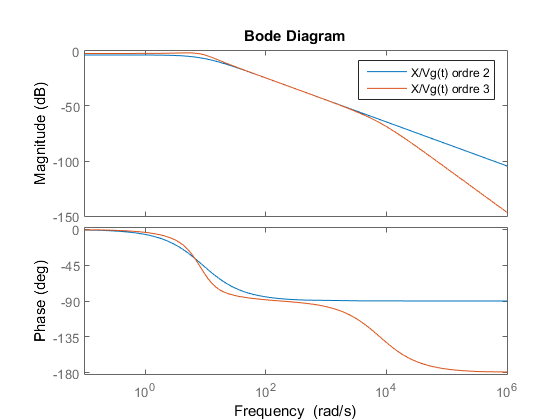
\includegraphics[scale=1]{./III/figure/bode_Tpert_EE1.png}
\captionof{figure}{Transfert des boucles fermées}

Le résultat que nous obtenons confirmes la stabilité asymptotique établie précédemment, cependant les différences notables avec le transfert du modèle d'ordre 2 en basse fréquence explique pourquoi nous n'avons pas pu respecter exactement le cahier des charges. 

\subsection{Changement de base du modèle d'ordre 4 et intégration de la commande}
De la même manière que pour le modèle d'ordre 3, nous effectuons un changement de base avec la matrice de passage : \begin{equation}
P = \begin{pmatrix}
0 &0& 1& 0\\ 0& 0& 0& 1\\1& 0& 0& 0\\ 0& 1& 0& 0
\end{pmatrix}
\end{equation}

Les performances du système bouclé ont les mêmes problèmes que pour le modèle d'ordre supérieur. Avec le même résultat pour l'erreur d'estimation que pour le modèle d'ordre 3, ces résultats était prévisible.

De plus, les approximations de modélisation ont montré dans l'analyse des modèles une erreur statique que nous ne pouvons pas corriger avec une commande construite sur le modèle d'ordre 2. Nous avons toutefois voulu analyser le transfert entre $Vg$ et la consigne et obtenons :
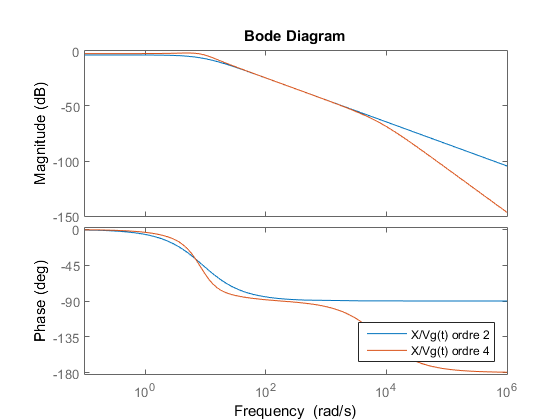
\includegraphics[scale=1]{./III/figure/bode_Tpert_EE0.png}
\captionof{figure}{Transfert des boucles fermées}
Nous avons de plus amples écart en basse fréquence avec un dépassement encore plus grand que pour le modèle d'ordre 3. Ce dépassement joue beaucoup sur les oscillations du système en boucle fermé. Le cahier des charges n'est encore une fois pas respecté pour ce modèle mais admet un temps de réponse proche de celui du modèle d'ordre 2.

En sachant ceci, nous savons que les dynamiques qui ont été simplifiés ne sont pas l'origine des écarts que nous venons d'exposer, il s'agit de la dynamique de l'observateur qui n'est pas très optimale. 

\subsection{Simulation SIMULINK}
Nous avons réutilisé la commande simulé précédemment pour l'implanter dans les modèles d'ordre 3 et 4. Ce prototypage rapide a eu les résultats suivant :
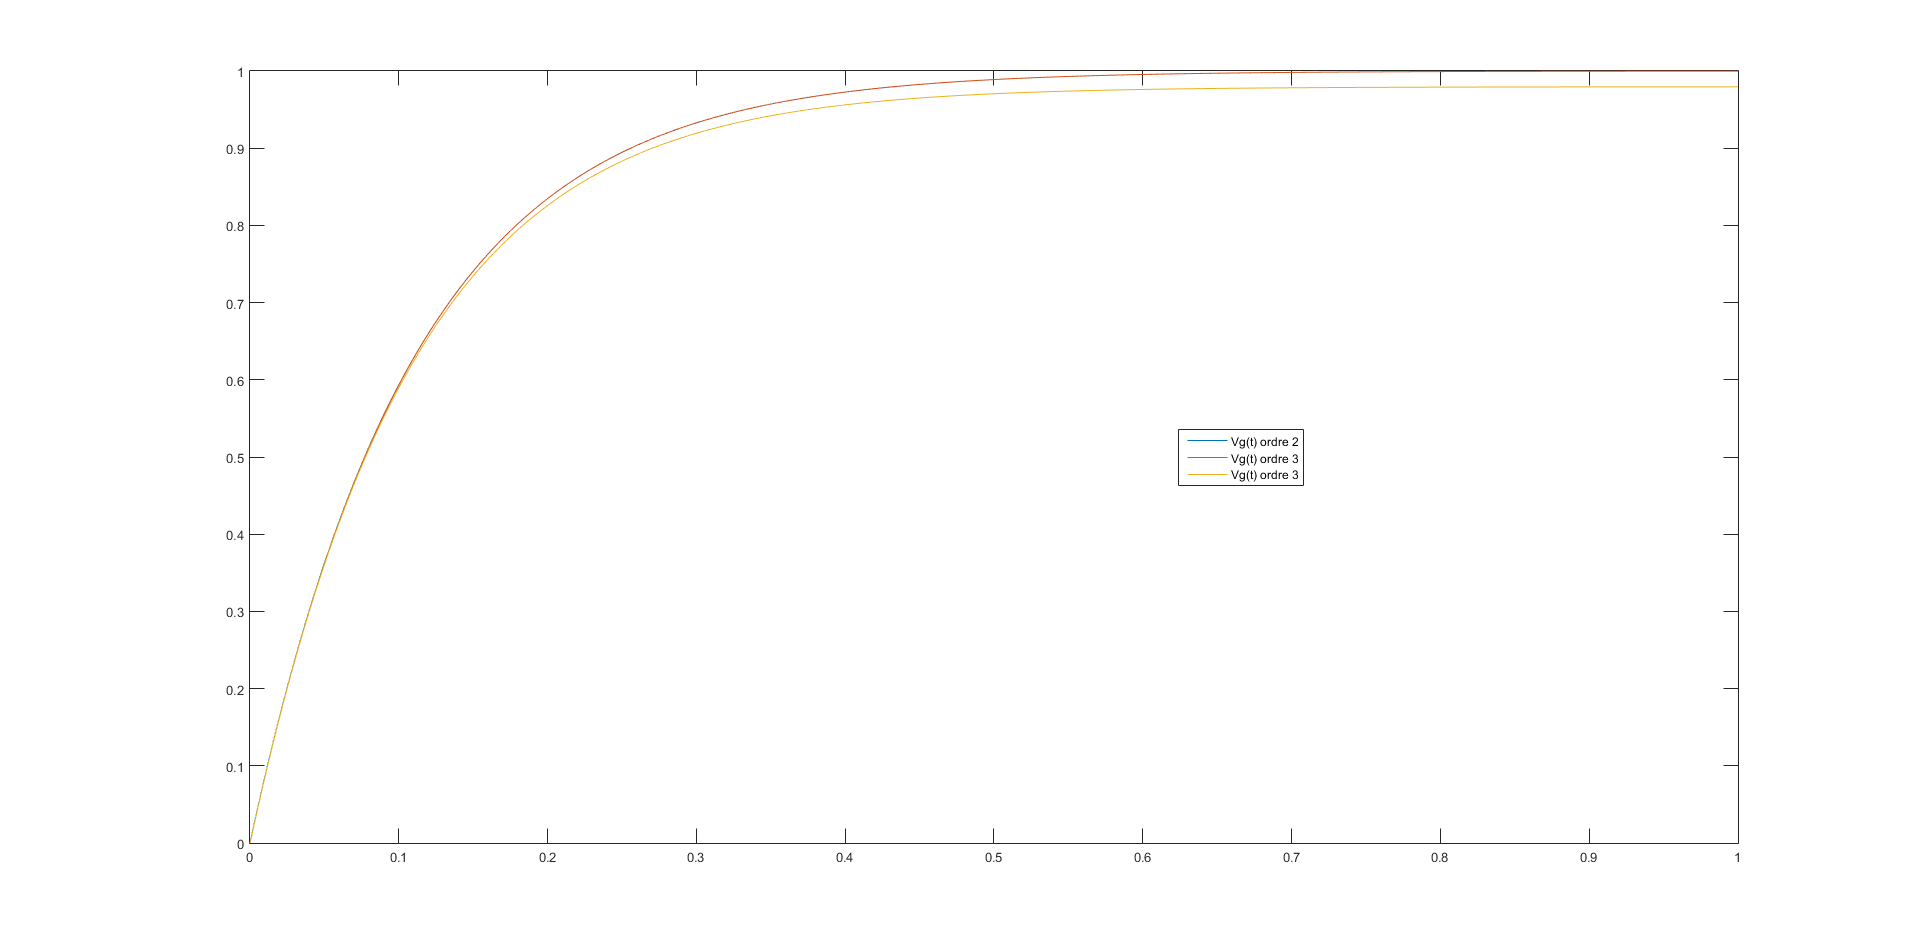
\includegraphics[scale=.3]{./III/figure/res_SIMULINK.png}
\captionof{figure}{Réponses temporelles des boucles fermées sous SIMULINK}
Ces résultats nous permettent de regarder une simulation des signaux de $Vg(t)$. D'après ces résultats, la commande que nous souhaitons appliquer respecte beaucoup mieux le cahier des charges que d'après l'analyse précédente. Cependant, nous ne pouvons en tirer aucune conclusion , il reste encore d'autres modèles plus complexes sur lequel notre commande doit être tester.


